\section{Gravitational Swarm Intelligence}
The Gravitational Swarm Intelligence Algorithm presented in this paper is a modified version of the algorithm presented in the paper "Gravitational Swarm for Graph Coloring" by Israel Carlos Rebollo Ruiz \cite{bib:GravSwarm}. Swarm Intelligence is a model where the emergent collective behavior is the outcome of a process of self-organization, where the agents evolve autonomously following a set of internal rules for their motion, interaction with the environment and the other agents. In this algorithm, the agents are subjected to an environment subject to a version of Newtonian Gravity. Centres of attraction (wells) are placed in the environment and the agents move based upon their attraction to these wells. Each well represents a distinct grouping or colouring of the underlaying graph. Agents experience a repulsive force if they try and enter a well already containing agents that prohibit a valid colouring. If an agent enters a well that is not prohibited, then it stops moving and takes on that well's colour. The algorithm ends once a set iteration limit is reached, or all agents settle into the wells, and hence a valid colouring is found.

\subsection{Implementation and Problems}
The action of each agent on every iteration is presented below:

\begin{figure}[H]
\caption{Agent logic for Gravitational Swarm}
\centering
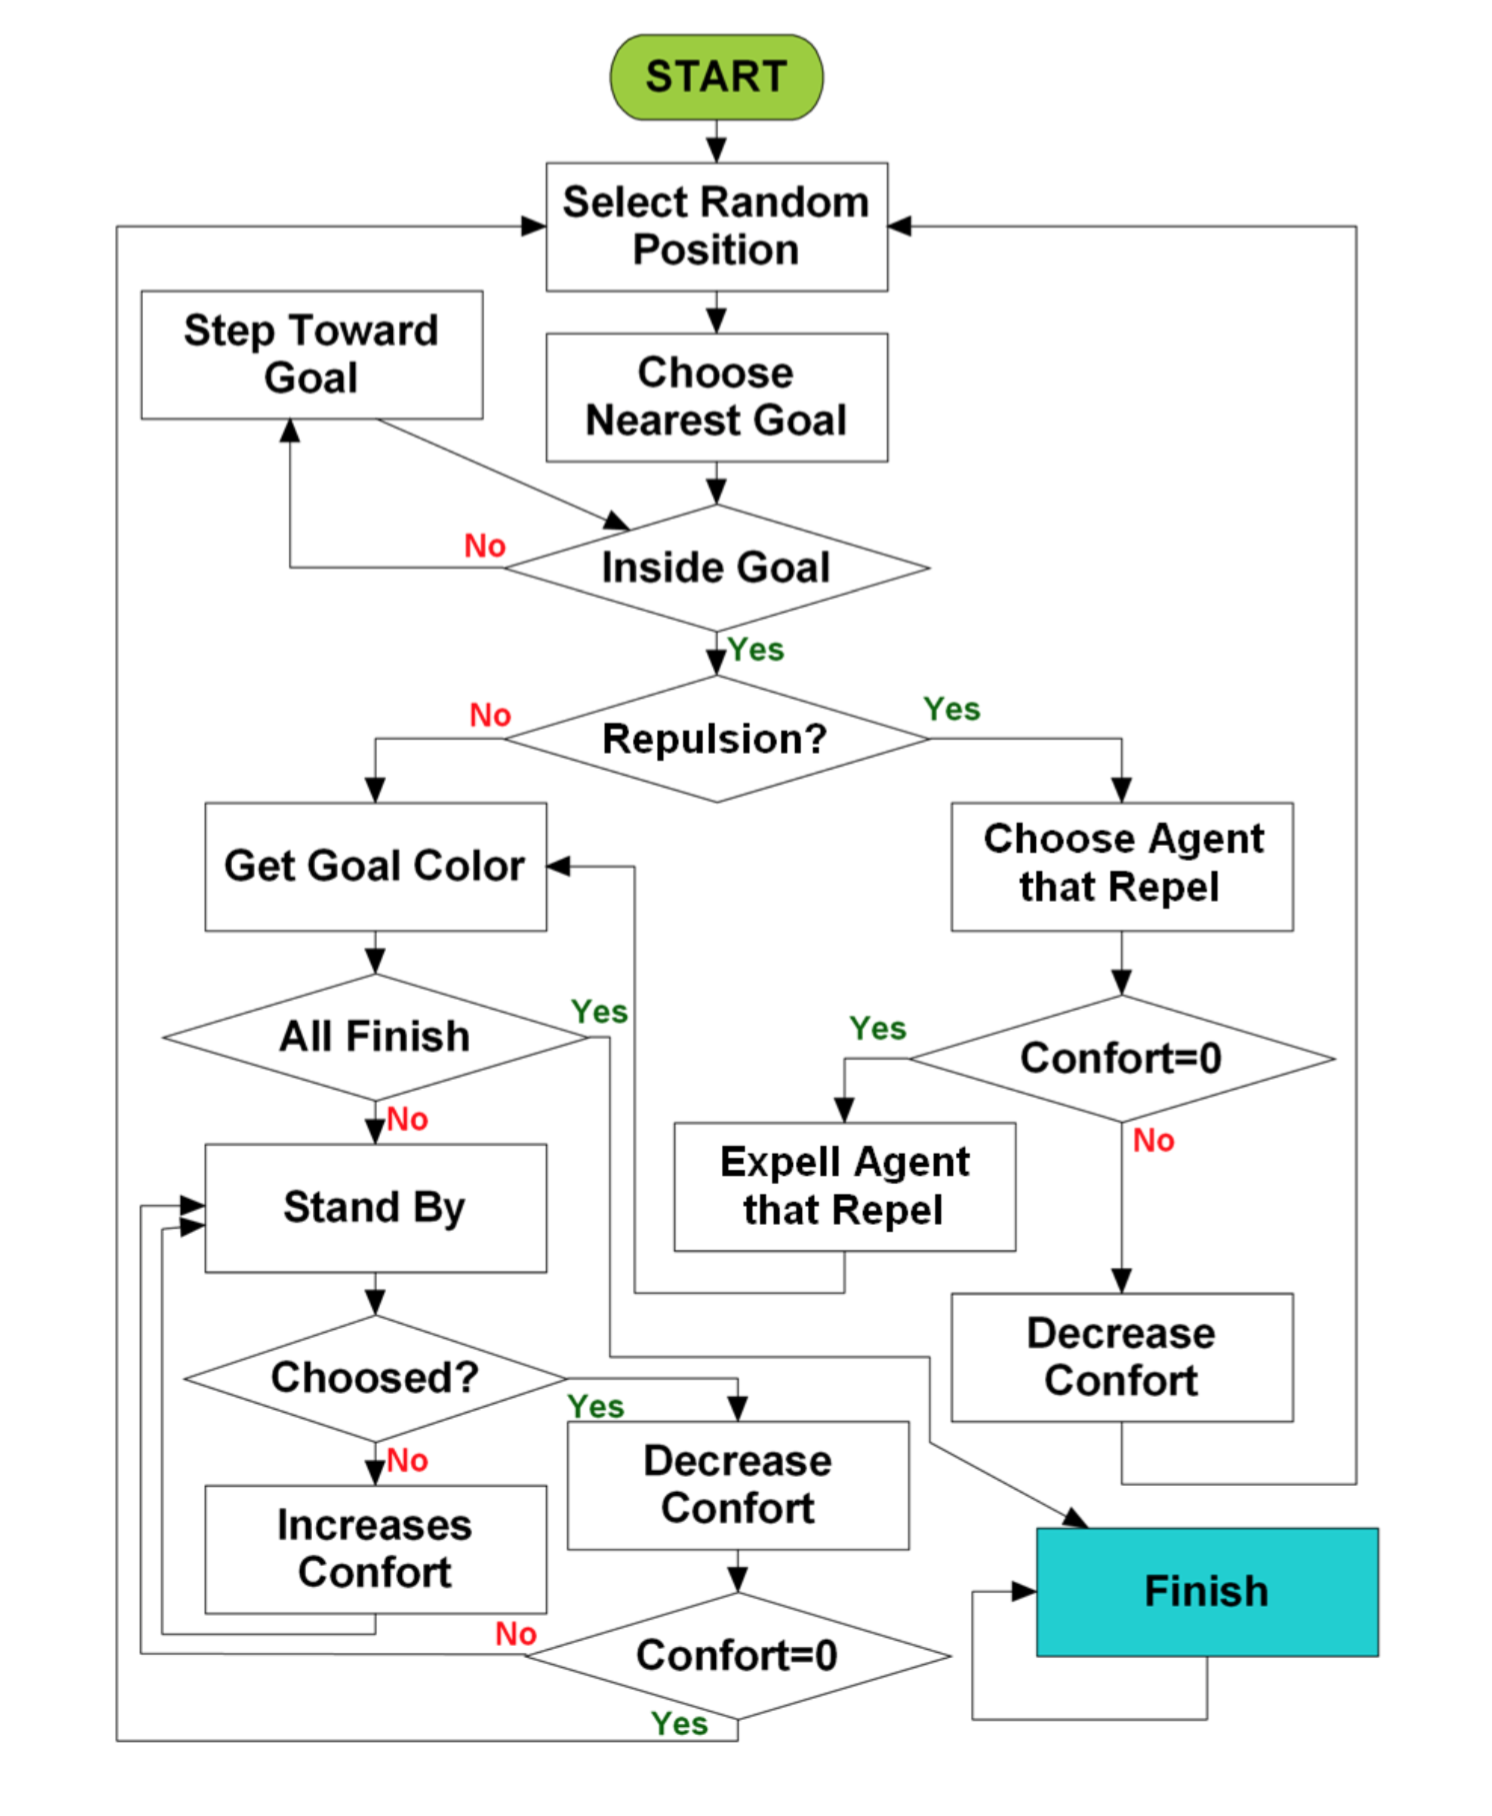
\includegraphics[width=\textwidth]{gs-cp-flow}
\end{figure}

Each agent moves in the toric world until all agents fall into the "Stand By" State. Then once the last agent triggers the "All Finished" State, the current colouring is accepted as valid. This algorithm presented some issues when implemented for testing. The comfort statistic that each agent tracks can grow unboundedly if the agents repeatedly fall into wells that they are subsequently repulsed from. This causes all captured agents to grow in comfort, making the local minuma harder to improve with every iteration and the chance of jumping out and finding a valid solution fall dramatically. 
\\The distance functions that were implemented were found to contain an error, resulting in a toroidal universe but gravitational attraction only in the plane. This meant that all results presented here use the non-toroidal distance. This does not present an issue, as the algorithm is still shown to converge to the solution as long as the distance functions work partially.
\\The figure below shows the location of wells within the universe, with distance functions permitting a toroidal universe. The colouring is a result of starting an agent at every possible start location and logging which well captures it. 
\begin{figure}[H]
\caption{Gravity mapping with gravity well locations overlayed}
\centering
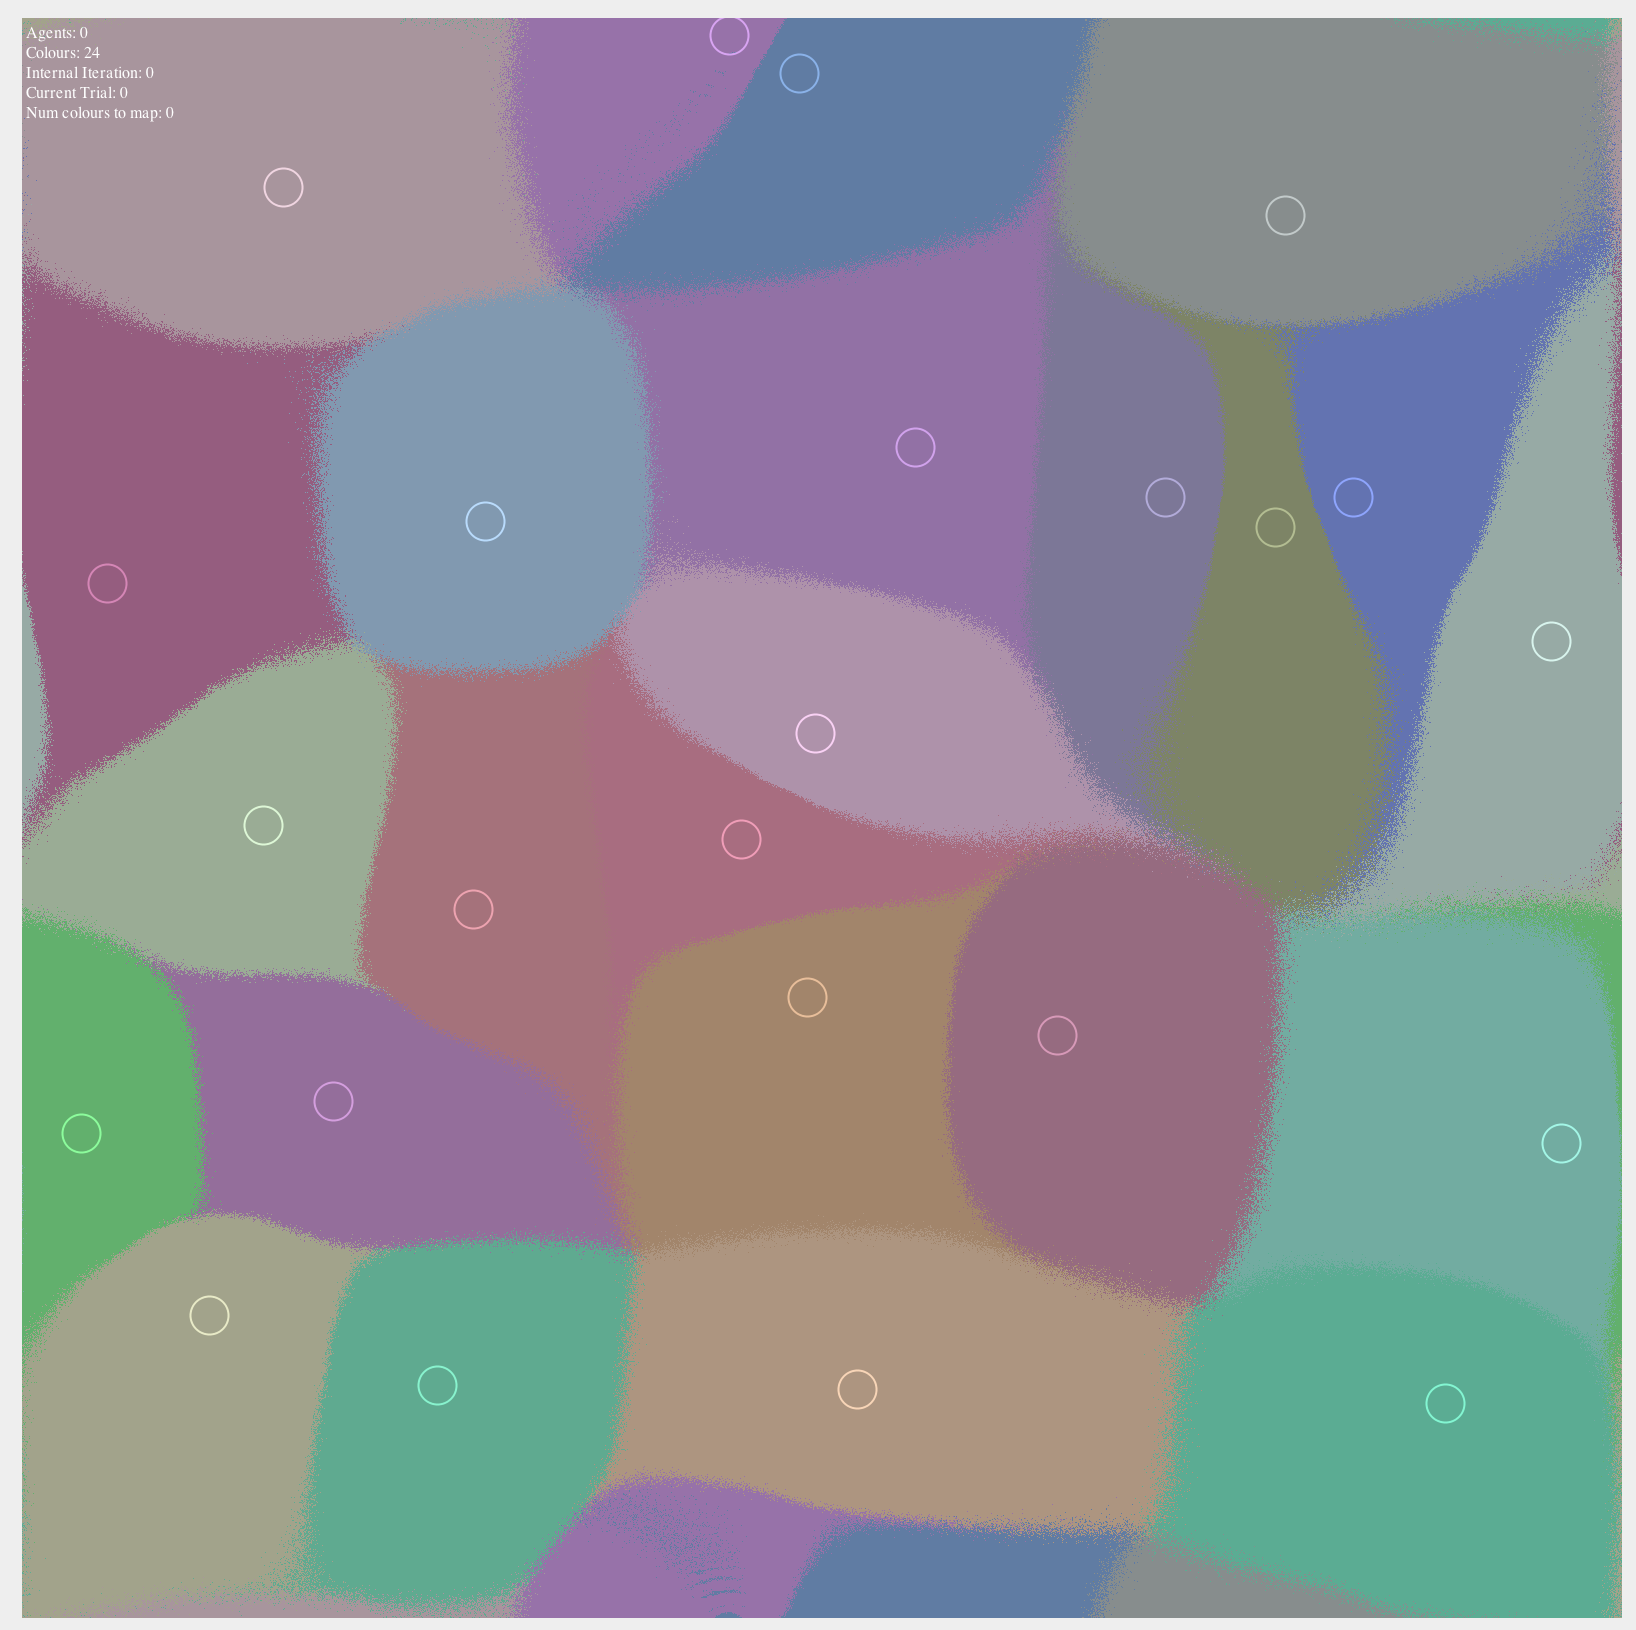
\includegraphics[width=\textwidth]{gradMapWithOverlay}
\end{figure}

\subsection{Workarounds}
This algorithm was relatively easy to implement, however much tweaking was required to ensure that the algorithm converges in a reasonable time and iteration count. The strength of the "gravity" had to be varied, and different radii of capture were compared, as these were the factors that caused the algorithm's runtime to be most affected. 

This algorithm was implemented from the psuedocode provided in \cite{bib:GravSwarm}, however the sample code omitted some details of the algorithm and instead presented these details the "Results and Observations" section of the paper. This lead to some aspects of the algorithm not functioning as intended. Interestingly, once the algorithm was tweaked to function correctly, the algorithm reflected the same observations that the original author had made. 

\subsection{Additions}
Substantial time and effort has been committed to the algorithm, with many aspects and details changing and growing over time to better solve the problems presented. The algorithm was trialled with the option for gravity wells to be able to take some "mass" from captured agents and have their own velocity in the universe. This addition did not increase the convergence rate of the algorithm but it did expose some flaws with the distance functions used to allow agents to track the wells. \\
Agent velocity and direction calculations have been changed and tweaked numerous times in the attempt to have agents move in the toroidal universe and react correctly to having multiple sources of strong attraction. To this end, a function was created that mapped agent start locations to final end points. Any "inconsistencies" are easily visually identified. An example of inconsistent behaviour is shown here:

\begin{figure}[H]
\caption{Toroidal Gravity Map with inconsistent behaviour - top left, top right exhibit "waterdrop" pattern}
\centering

\includegraphics[width=\textwidth]{GradMap1445410689515}
\end{figure}

The large amounts of variability around disputed boundaries is a result of the random noise added to the velocity on every iteration. It was found that if no noise was added, when there was very low gravity values (an agent was a long distance from \emph{any} well), the agent would stall, taking many iterations to gain speed and be captured. The random noise helps to speed up the process, and can reduce the amount of iterations in a stall by "randomly walking" around the region until the gravity values become larger than the random noise. 
